% arara: pdflatex
% !arara: indent: {overwrite: yes, localSettings: yes}
\documentclass{beamer}
\usepackage[latin1]{inputenc}
\usetheme{Boadilla}
\usecolortheme{seagull}
\usefonttheme{structurebold}
\usepackage{standalone}
\usepackage{tikz}
\usetikzlibrary{positioning}
\usetikzlibrary{mindmap}
\usetikzlibrary{decorations.text}
\usetikzlibrary{shapes}

% global tikz settings
\tikzset{
   % reveal mindmap step by step
   % http://tex.stackexchange.com/questions/55806/mindmap-tikzpicture-in-beamer-reveal-step-by-step
   invisible/.style={opacity=0},
   visible on/.style={alt=#1{}{invisible}},
   alt/.code args={<#1>#2#3}{%
      \alt<#1>{\pgfkeysalso{#2}}{\pgfkeysalso{#3}} % \pgfkeysalso doesn't change the path
   },
   % clouds for the time line diagram
   cloudy/.style={
      cloud,
      draw=gray,
      double,
      thick,
      align=center,
      aspect=3.3,
      cloud puffs=10,
   },
}

% stars
\pgfdeclaredecoration{stars}{initial}{
   \state{initial}[width=15pt]
   {
      \pgfmathparse{round(rnd*100)}
      \pgfsetfillcolor{yellow!\pgfmathresult!orange}
      \pgfsetstrokecolor{yellow!\pgfmathresult!red}
      \pgfnode{star}{center}{}{}{\pgfusepath{stroke,fill}}
   }
   \state{final}
   {
      \pgfpathmoveto{\pgfpointdecoratedpathlast}
   }
}


% image paths
\graphicspath{{images/}}

% title information
% title information
% title information
\title[WeBWorK]{WeBWorK---a Faculty-driven Homework Management System}
\author[Jordan, Hughes, Yao]{Alex Jordan \and Chris Hughes \and Xiaolong Yao}
\institute[PCC]{Portland Community College}
\date{February 17, 2014}

%\includeonlyframes{wwhistory}
\begin{document}

\begin{frame}
   \tikz [remember picture,overlay]
   \node[opacity=0.1] at
   %([yshift=3cm]current page.south)
   (current page.center)
   {
\includegraphics[width=.75\textwidth]{WeBWorK-logo-tikz}};
   \titlepage
\end{frame}

\begin{frame}
   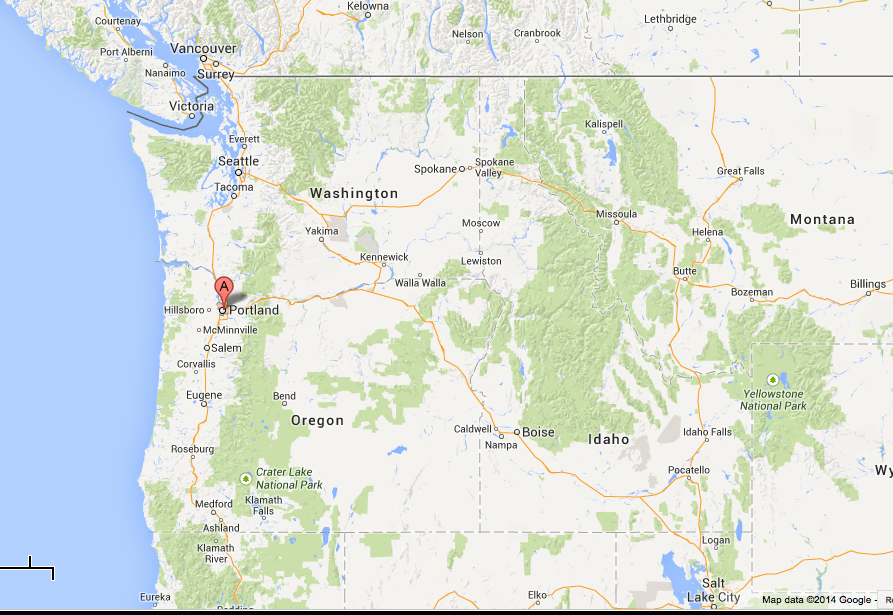
\includegraphics[width=\textwidth]{map}

\end{frame}

\begin{frame}
\begin{block}{WeBWorK at PCC login}
\centering
\url{http://webwork.pcc.edu}

\begin{description}
\item[Course:] eLearning2014
\item[Username:] a1--z9 (lowercase!)
\item[Password:] pass (lowercase!)
\end{description}

\end{block}
\end{frame}

\begin{frame}[label=wwhistory]{WeBWorK history}

\begin{tikzpicture}
    %draw horizontal line
    \draw (-2,0) -- (10,0);

    %draw vertical lines
    \foreach \x in {-1.5,3,8}
    \draw (\x cm,3pt) -- (\x cm,-3pt);

    %draw nodes
    \draw (-1.5,0) node[above=3pt] {$\sim$1995--2003};
    \draw (3,0) node[above=3pt] {2003--2011};
    \draw (8,0) node[above=3pt] {2011--present};

\end{tikzpicture}
\small
\begin{columns}[t]
    \begin{column}{.33\textwidth}
        \begin{itemize}
		\item[95] Arnie Pizer and Mike Gage at University of Rochester inspired by CAPA
		\item[96] WeBWorK named, first courses taught
		\item[97] used outside of Rochester %at Johns Hopkins first 
		\item[02] Perl4$\to$Perl5, version control begins
        \end{itemize}
    \end{column}%
    \hfill\pause
    \begin{column}{.33\textwidth}
        \begin{itemize}
        		\item[03] WeBWorK 2:  Math Objects, quizzes, jsMath, more
		\item[05] National Problem Library
		\item[07] Moodle compatibility
		\item[09] MathJax opens accessibility doors
            	\item[10] MAA grant to disseminate
        \end{itemize}
    \end{column}%
    \hfill\pause
    \begin{column}{.33\textwidth}
        \begin{itemize}
        		\item[11] git repository and development accelerates:\\
		WeBWorK 2.6 %configuration files, Math Achievements, more
		\item[12]  WeBWorK 2.7 %essay answers, bootstrap CSS, equation editor, more
		\item[13]  WeBWorK 2.8 % improved instructor interface, OPL, much more
		\item[14] initial sketching of WeBWorK 3 is underway
        \end{itemize}
    \end{column}
\end{columns}
\end{frame}
%----------------------------------------------------------------------------------------------------------------------------------------------------------------
\begin{frame}{Servers in North America}
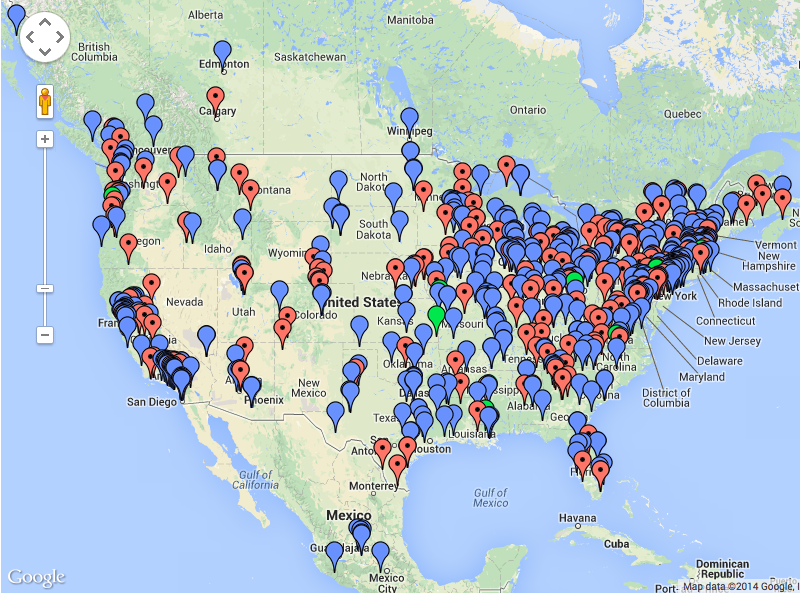
\includegraphics[width=\textwidth]{mapUS}
\end{frame}

\begin{frame}{Servers all over the world}
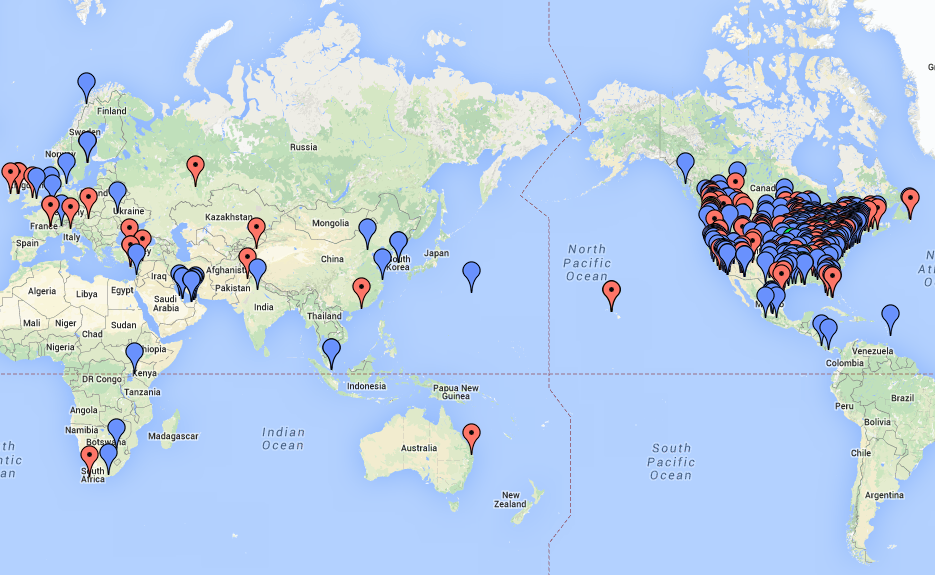
\includegraphics[width=\textwidth]{mapWorld}

\end{frame}

%----------------------------------------------------------------------------------------------------------------------------------------------------------------

\begin{frame}[label=timeline]{PCC's journey\ldots}
   \begin{tikzpicture}
         % Spring 2010
         % Alex joins PCC and starts using WeBWorK on his own-
         % he spoke to Holli Adams (department chair at the time)
         % and arranges to have courses hosted at Rochester
         \node[cloudy](spring2010){Spring 2010};
         \node[below=0mm of spring2010]{
\includegraphics[width=1cm]{firststep}};
      \pause
         % Summer 2010
         % Alex codes problems from our current text books for
         % MTH 60, 65, 95 single handedly
         \node[cloudy,right=of spring2010](summer2010){Summer 2010};
         \node[below=0mm of summer2010]{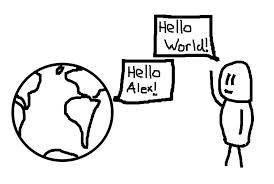
\includegraphics[width=3cm]{alexcodes}};
      \pause
         % Fall 2010
         % Alex makes arrangements with University of Oregon
         % and a small number of faculty joined him in using WeBWorK
         \node[cloudy,right=of summer2010](fall2010){Fall 2010};
         \node[below=0mm of fall2010](uofo){
\includegraphics[width=3cm]{universityoforegon}};
      \pause
         % Winter 2011
         % Alex and Chris contacted Tammy- they were too busy with
         % migration to gmail; they rejected us
         \node[cloudy,below=-.1cm of uofo](winter2011){Winter 2011};
         \node[below=0mm of winter2011]{
\includegraphics[width=3cm]{emailtss}};
      \pause
         % Fall 2011
         % PCC starts targetting Accessibility- administrative buzz word
         % at every meeting
         \node[cloudy,left=of winter2011](fall2011){Fall 2011};
         \node[below=0mm of fall2011]{
\includegraphics[width=3cm]{access}};
      \pause
         % Fall 2012
         % Chris and Scot get release time to study accessibility,
         % and introduce Alex to Karen and Kaela; the world of PCC changes.
         %
         % During this time period (Spring 2010-Fall2012) there is an
         % increased presence of MML; accessibility tests failed in Fall 2012
         \node[cloudy,left=2cm of fall2011](fall2012){Fall 2012};
         % every administrator now starts to listen to Alex's e-mails
         % about WeBWorK
         \pause
         \node[below=0mm of fall2012]{
\includegraphics[width=3cm]{listening}};
   \end{tikzpicture}
\end{frame}

\begin{frame}[label=support]{Support}
   \begin{tikzpicture}
      % Winter 2013
      % We received official support to move forward with our own server:
      % webwork.pcc.edu
      \node[cloudy](winter2013){Winter 2013};
      \node[below=0mm of winter2013]{
\includegraphics[width=3cm]{handshake}};
      \pause
         % Spring, Summer 2013
         % Alex, Carl, and Chris coded furiously to complete
         % MTH 60 and 65 problems; sadly there was not enough time for
         % MTH 95
         \node[cloudy, right=of winter2013](summer2013){Summer 2013};
         \node[below=0mm of summer2013]{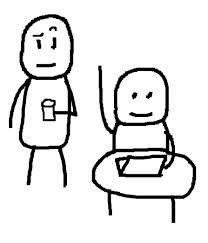
\includegraphics[width=3cm]{collaboration}};
      \pause
         % Fall 2013
         % Alex, Carl and Chris announce their success to the SAC,
         % which is very shortly followed by an EPIC crash on the UO server
         \node[cloudy,fill=green, right=of summer2013](fall2013){Fall 2013};
\pause
         \node[xshift=-0.8cm,yshift=-1.7cm,right=of summer2013]{
\includegraphics[width=3cm]{lightning}};
         \node[cloudy,fill=green,draw=red, right=of summer2013](fall2013){Fall 2013};
   \end{tikzpicture}
\end{frame}

\begin{frame}[label=success]{Success}
   \centering
   
\begin{tikzpicture}
      % Winter 2014
      % webwork.pcc.edu goes live, and works wonderfully well
      \node[star,very thick, double,fill=yellow,draw=orange](winter2014) {Winter 2014};;
      \path[decorate, decoration=stars, star point ratio=2, star points=5,
         inner sep=0, minimum size=rnd*10pt+2pt]
         circle (3cm);
   \end{tikzpicture}
   \href{https://webwork.pcc.edu/webwork2/}{https://webwork.pcc.edu/webwork2/}
\end{frame}

\begin{frame}[label=definition]
   \centering
   \resizebox{.87\textwidth}{!}{%
      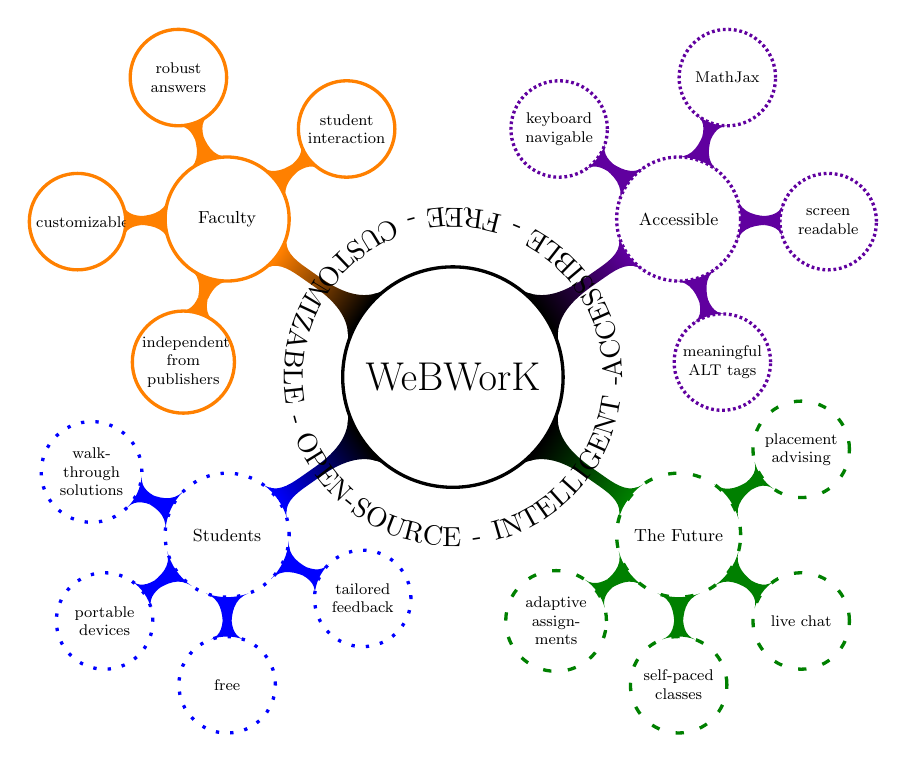
\begin{tikzpicture}[mindmap,
            concept/.append style={fill={none}},
            root concept/.style={concept color=blue},
            level 1 concept/.append style=
            {level distance = 35mm},
            level 2 concept/.append style=
            {level distance = 19mm},
            every node/.append style={align=center,scale=0.7},
         ]
         \node [concept,font=\huge] {WeBWorK}
         child[grow=145, concept color=orange,visible on=<2->] {node[concept] {Faculty}
            child[grow=37, visible on=<2->]{node[concept] {student interaction}}
            child[grow=109, visible on=<2->]{node[concept] {robust\\ answers}}
            child[grow=181, visible on=<2->]{node[concept] {customizable}}
            child[grow=253, visible on=<2->]{node[concept] {independent from publishers}}
         }
         child[loosely dotted,concept color=blue,grow=215,visible on=<3->] {node[concept] {Students}
            child[grow=155,visible on=<3->]{node[concept] {walk-through solutions}}
            child[grow=215,visible on=<3->]{node[concept] {portable\\devices}}
            child[grow=270,visible on=<3->]{node[concept] {free}}
            child[grow=335,visible on=<3->]{node[concept] {tailored feedback}}
         }
         child[dash pattern=on 1pt off 1pt on 1pt off 1pt, concept color=blue!50!purple,grow=35,visible on=<4->] {node[concept] {Accessible}
            child[grow=143,visible on=<4-> ] {node[concept] {keyboard navigable}}
            child[grow=71,visible on=<4->] {node[concept] {MathJax}}
            child[grow=359,visible on=<4->] {node[concept]{screen\\ readable} }
            child[grow=287,visible on=<4->] {node[concept] {meaningful ALT tags}}
         }
         child[loosely dashed,concept color=green!50!black,grow=325,visible on=<5->] {node[concept] {The Future}
            child[grow=215,visible on=<4-> ] {node[concept] {adaptive assignments}}
            child[grow=35,visible on=<4->] {node[concept] {placement advising}}
            child[grow=270,visible on=<4->] {node[concept] {self-paced classes}}
            child[grow=-35,visible on=<4->] {node[concept] {live chat}}
         };
         \node at (0,0) [inner sep=15mm,decorate,circle,decoration=
            {raise=10pt,text along path,text={ACCESSIBLE - FREE - CUSTOMIZABLE - OPEN-SOURCE -  INTELLIGENT - },
               text align=fit to path,
            }] {};
      \end{tikzpicture}
   }
\end{frame}


\end{document}



% some junk I was trying with the success frame
%\path[decorate, decoration=stars, star point ratio=2, star points=5,
%inner sep=0, minimum size=rnd*10pt+2pt]
%(winter2014.north west) .. controls (-3,2) and (-4,2) .. (-5,0)
%.. controls (-3,0) and (-3,-1) .. (-4,-3)
%.. controls (-2,-5) and (-1,-5) .. (0,-2)
%.. controls (2,-5) and (1,-5) .. (4,-3);
